
\lhead[\leftmark]{\leftmark}

\rhead[\leftmark]{}

\lfoot{}

\cfoot[\thepage]{\thepage}

\chapter{Introduction and Literature Review}

\section{A Solution to Offline Dating Limitations\label{sec:A-Solution-to}}

\lettrine{T}{he}{ rise of the Internet and its effects on behaviour are undeniably
pervading across all social strata. Online dating can be considered
one of the foremost examples of a fundamentally altered social activity
in the modern Internet era: finding a partner nowadays can be accomplished
through Computer-Mediated Communication (CMC) in a faster \textendash{}
and usually more efficient \textendash{} way with respect to traditional
meeting venues. The Internet allows for free and instant access to
worldwide information, going beyond the limits of physical space and
time of offline activities. The same concept applies to Online Dating
which, contrary to conventional meeting venues with soundly structured
social spheres, allows its users to surpass social class, time and
even geographical barriers.}

This work is grounded in the assumption that the emergence of online
dating is a natural consequence of the modernisation processes that
lead to the rationalisation, marketisation\footnote{Please note that the marketisation of love and intimacy has not started
with online dating. In fact, as \citet{Schmitz2016The-Structure-o}
points out, common meeting venues have gradually shifted from family
and neighbourhood to more explicit partner markets (like nightclubs)
from the 50s onwards. } and ultimately to the \textquotedblleft commodification of romance\textquotedblright{}
\textendash{} i.e., of choosing potential mates \citep{Illouz1997Consuming-the-R}
\textendash{} that is quintessentially Western culture. This is reflected
in the increasing significance of online dating in daily life, easily
ascertainable by each own personal experiences. Official data on the
usage of online dating apps is often unavailable mainly due to privacy
concern, but it is out of doubt that online dating is penetrating
all social classes and age groups: one in three marriages in the U.S.
now\footnote{This could be an underestimation, since data from 2013 are probably
outdated nowadays. } begins online \citep{Cacioppo2013Marital-satisfa}. Match Group,
owning a portfolio of more than 45 online dating brands \textendash{}
including Tinder, the most downloaded dating mobile app worldwide
\textendash{} reported \$1.3 billion revenues in 2017 and boasts a
current market capitalisation of \$10.5 billion\footnote{Financial data retrieved from Bloomberg and Q1 2018 Investor Presentation
of Match Group. }. These data can be considered a proxy measure of this rapidly growing
industry and a signal of these emerging social phenomena. Analysing
the online partner market seems crucial to retrieve insights on usage,
behaviours and mate choice preferences, especially since these new
tools can shape how people date or fall in love in the digital era
and hence the demography of our communities. Not only that, online
dating can also help in surpassing the classical (micro-)economic
theories of mate selection rooted in the pre-Internet era \citep{Becker1991A-Treatise-on-t},
when the problem of search in mate selection had no clear answers
due to the absence of proper data \citep{Michael-J.-Rosenfeld2012Searching-for-a}.
Hence this work aims at providing a better understanding of the online
partner market, and it is structured as follows: firstly, an introduction
to online dating seen as an efficient solution to the issues of offline
partner markets is elaborated; secondly, theories on its functioning
\textendash{} as a marketplace in particular \textendash{} are discussed
and its main characteristics are outlined; finally, an empirical analysis
is run on a 2,001 U.S. adults data set, in order to shape common online
dating user profiles and assess the determinants of its usage. 

Online dating can be defined as the practice of using Internet to
find a short-term sexual or a long-term romantic partner. Thereby
an online dating platform is a website or mobile app that allows its
users to find their best possible partner, through presenting themselves
usually with a short biography, photos and other kinds of information,
contacting potential mates via chat and picking promising profiles
out of a large pool of contacts. Although different models can be
identified, most online dating websites and mobile apps can be traced
back to two main functioning standards that will be analysed later
on (see \prettyref{subsec:Matchmaking-and-Scroll-based}). Often,
very little differentiation can be found among them; however new trends
of niche apps are emerging, with different concepts and targeting
different market segments \textendash{} homosexual dating, elderly
dating, religious dating, etc. By definition, online dating could
be extended to other websites and mobile apps like Facebook, as people
could potentially flirt or fall in love on platforms with a great
variety of purposes; for the sake of simplicity, in this work we will
only consider and refer to dating platforms that have been intentionally
designed for this very purpose. It is important to notice that all
the concepts apply both to online dating and mobile dating, as the
difference between the two is becoming negligible (thus we will only
refer to \textquotedblleft online dating\textquotedblright{} in general
from now on): as roughly 57\% of Internet traffic comes from mobile
and tablet devices nowadays\footnote{Data retrieved from \citet{BrightEdge201757-of-Search-Tr}.},
more and more people expect a mobile version of desktop websites as
well as a mobile app, inducing dating services to become ubiquitous.

People used to meet their partners through mutual friends, workplace,
church, neighbourhood, school and family. In the last 15-20 years,
the Internet has partially displaced those conventional offline mating
venues. It is common for people to partner with complete strangers\footnote{That is to say with people to which they had no social ties previously. }
nowadays, as a consequence of the increased efficiency brought about
by online dating platforms \citep{Michael-J.-Rosenfeld2012Searching-for-a}.
This unprecedented search efficiency is particularly convenient to
those singles\footnote{The definition of \textquotedblleft single\textquotedblright{} is
a rather vague. For the sake of simplicity, and unless otherwise noted,
in this work we will adopt the statistical definition, which simply
means unmarried, but leaves out plenty of family structures \textendash{}
e.g., couples.} who would otherwise lack an easy access to the partner market (see
\prettyref{fig:The-Changing-Way}).

\begin{figure}[h]
\includegraphics[width=1\columnwidth]{assets/rosenfeld1}

\caption{The Changing Way Americans Meet Their Partners\label{fig:The-Changing-Way}\protect \\
{\footnotesize{}N = 2,462 for heterosexual couples, N = 462 for same-sex
couples.}\protect \\
{\footnotesize{}\textquotedblleft Individuals who face a thin market
for potential partners, such as gays, lesbians, and middle aged heterosexuals,
are especially likely to meet partners online.\textquotedblright }\protect \\
{\footnotesize{}Source: \citet{Michael-J.-Rosenfeld2012Searching-for-a}.}}
\end{figure}

As social class and geographical barriers are often reduced by the
way online dating platform are designed, their users can realise their
preferences more efficiently. The effects of rationalisation and the
intrusion of market-driven logics on intim
acy and cyberdating lead
the modern user to take everyday decisions based on cost-benefit ratios.
User's actions on digital dating platforms are often driven by their
own preferences and rational intentions. When compared to more traditional
meeting venues \textendash{} commonly based on structured social spheres\footnote{For example: bars and restaurants, schools, nightclubs and churches
are often frequented by different people. Each meeting venue is usually
frequented by a socially homogeneous group of people. } \textendash{} online dating appears strongly influenced by market
principles: exchange logics, objectification and competition for potential
partners, a large base of \textquotedblleft suppliers\textquotedblright ,
lower transaction costs and conscious rational mate choices make it
metaphorically similar to a marketplace \citep{Schmitz2016The-Structure-o}.
As a matter of fact, it can be considered rather close to the \textquotedblleft ideal-typical\textquotedblright{}
partner market from an economic standpoint. In addition to this, online
dating can be interpreted as a promising tool to demolish gender roles
and norms: \citet{Scharlott1995Overcoming-Rela} argue that \textquotedblleft the
safety and anonymity the system offered\textquotedblright{} allows
online daters to \textquotedblleft break free from traditional sex
role norms\textquotedblright . 

Following the realisation that these platforms are designed with the
precise goal of efficient partner choice, some see the intrusion of
market logics as \textquotedblleft emotional capitalism\textquotedblright ,
a rationalist threat to true romance that ultimately should not have
economic motives \citep{Illouz2007Cold-Intimacies}. However, in this
paper the author tries to apply a value-free and unbiased perspective
both to traditional and online dating concepts.


\section{Early Stages in Social Network Analysis}

In pursuance of explaining the efficiency gains that are said to be
a strength of online dating, we start by deepening further the social
network analysis.

In one of his well-known books, \citet{J.1934Who-Shall-Survi} theorised
the \textquotedblleft sociogram\textquotedblright{} as a tool to represent
the formal properties of social configurations, built with diagrams
whereby individuals are represented by points in space and their social
relationships by lines. Nowadays this concept is well established
and commonly used in academia. The concept of \textquotedblleft balance\textquotedblright{}
was later introduced in the sociogram after the development of the
balance theory by \citet{Heider1946Attitudes-and-c}. He argues that
congruence among attitudes with other people is fundamental in order
to achieve cognitive balance. That is to say that \textit{ego's} balance
is achieved only if in a set of attitudes towards people (\textit{alter}),
they are all similar in their sign \textendash{} i.e., all attitudes
are either positive or negative, at their simplest. In other words,
given the fact that a person $A$ likes\footnote{Likes, loves, values or approves, as \citet{Cartwright1956Structural-Bala}
put it. } the person $B$ and the person $B$ likes the person $C$, balance
in the triad is achieved only if $A$ likes $C$ as well. The concept
of cognitive balance was later extended at interpersonal level in
social groups, thus allowing researchers to study whole structures
simultaneously and not from one \textit{ego's} point of view at a
time. A new framework developed by \citet{Cartwright1956Structural-Bala}
builds on Moreno's work and applies the concepts of graph theory to
the sociogram. They argue that the lines representing the relations
among individuals in a graph could be provided with a sign + or \textendash{}
to indicate either a positive or a negative relation and an arrow
to illustrate the direction of such relationship. For instance, it
is possible to indicate that person $A$ has a positive relation with
person $B$ ($A$ likes $B$, or $A\mathit{\mathbf{L}B}$) but person
$B$ has a negative relation with person $A$ ($B$ dislikes $A$,
or $B\mathbf{\sim L}A$). In the case of triadic relationships, the
balanced state can be achieved only if all relations are positive,
or if two are negative and one is positive. Thus $(A\mathit{\mathbf{L}B},\,B\mathit{\mathbf{L}C,\,A\mathit{\mathbf{L}C)}}$,
$(A\mathit{\mathbf{\sim L}B},\,B\mathit{\mathbf{\sim L}C,\,A\mathit{\mathbf{L}C)}}$
are examples of balanced triads, while $(A\mathit{\mathbf{L}B},\,B\mathit{\mathbf{L}C,\,A\mathit{\mathbf{\sim L}C)}}$
is not (see \prettyref{fig:Some-structures-examples.The}). In undirected
graphs (with no arrows) the relationships between A and B and between
B and A are considered to be equal or perfectly reciprocal. This results
in a (un)balanced state given only by the signs attached to the relations
in the graph, irrespectively of the directions of such relations.
\begin{figure}[h]
\begin{centering}
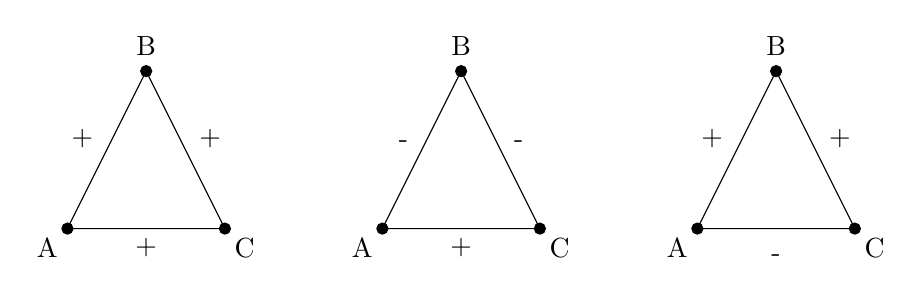
\begin{tikzpicture}
\filldraw (0,0) circle (2pt) node[below left] {A} -- (1,2) circle (2pt) node[pos=0.45,above left] {+} node[above=2pt] {B} -- (2,0) circle (2pt) node[pos=0.55,above right] {+} node[below right] {C} -- (0,0) node[midway,below] {+};
\filldraw (4,0) circle (2pt) node[below left] {A} -- (5,2) circle (2pt) node[pos=0.45,above left] {-} node[above=2pt] {B} -- (6,0) circle (2pt) node[pos=0.55,above right] {-} node[below right] {C} -- (4,0) node[midway,below] {+};
\filldraw (8,0) circle (2pt) node[below left] {A} -- (9,2) circle (2pt) node[pos=0.45,above left] {+} node[above=2pt] {B} -- (10,0) circle (2pt) node[pos=0.55,above right] {+} node[below right] {C} -- (8,0) node[midway,below=4pt] {-};
\end{tikzpicture}
\par\end{centering}
\centering{}\caption{Some triadic structures examples.\label{fig:Some-structures-examples.The}}
\end{figure}
These triads are of particular importance. According to \citeauthor{Cartwright1956Structural-Bala},
actual and intricate social structures can be imagined as being composed
of overlapping simple triads. Hence these triads are the elementary
units of more complex social structures seen in real life, and should
be analysed in order to infer the properties of complex networks.
For instance, a large network is balanced if all its elementary triads
are balanced. Large interpersonal networks can be studied with a great
variety of metrics. In his social network development analysis, \citet{Scott1991Social-Network-}
gathers and classifies these metrics following the codification work
of \citet{Mitchell1969Social-Networks}. For the sake of this work
we put emphasis on \textit{homophily}, that is the extent of actors
to forge relationships with (dis)similar individuals; \textit{propinquity},
the propensity to tie with physically close actors;\textsl{ }\textit{reciprocity},
the degree to which actors are mutually interested and interact with
each other;\textsl{ }\textit{intensity}, that refers to the strength
of obligations arisen in a relationship; \textit{density}, which stands
for the proportion of ties present in a network compared to the number
of all potentially possible ties \textendash{} i.e., the completeness
of the network.

In the next section we build on these foundations to elaborate efficiency
theories based on the strength of ties in social networks.

\section{Weak and Absent Ties Hypotheses}

Strength is another essential characteristic of interpersonal ties
in social networks. \citet{Granovetter1973The-Strenght-of} defines
the tie strength as:

\begin{spacing}{1}
\begin{quotation}
\textquotedblleft a (probably linear) combination of the amount of
time, the emotional intensity, the intimacy (mutual confiding), and
the reciprocal services which characterise the tie\footnote{Assuming positive and symmetric ties.}.\textquotedblright{}
\end{quotation}
\end{spacing}

Consequently, three main categories of tie strengths can be identified:
strong ties, weak ties and absent ties. Typically a strong tie is
correlated with high degrees of homophily and propinquity, as opposed
to weak ties that serve as \textquotedblleft bridges\textquotedblright{}
between clumps of individuals with strong ties. Starting from his
revolutionary \textquotedblleft The Strength of Weak Ties\textquotedblright ,
\citet{Granovetter1973The-Strenght-of} radically influenced the concept
of ties in social networks, posing particular attention to weak and
absent ties\footnote{Those ties with no particular significance: e.g., the neighbour you
wave when back home. }. The weak tie hypothesis suggests that, according to probability
reasoning, if $A$ has a strong tie both with $B$ and $C$, then
a (probably weak) tie between $B$ and $C$ is also present \textendash{}
or is very unlikely to be absent (see Figure \ref{fig:Weak-tie-in}).
If that was not the case, a \textit{forbidden triad} would arise\footnote{Imagine that person $A$ likes and values the celebrity $B$. If $B$
likes and endorses a product $C$, then it is very likely that $A$
will start liking $C$ as well \textendash{} or disliking $B$ \textendash{}
to achieve balance. }. 

\begin{figure}[h]
\begin{centering}
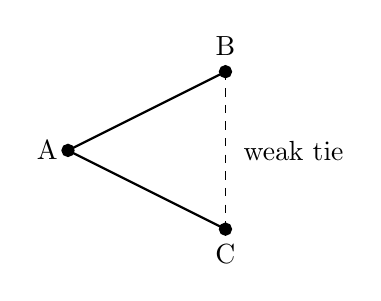
\begin{tikzpicture}
\filldraw[thick] (2,0) circle (2pt) node[below=2pt] {C} -- (0,1) circle (2pt) node[left] {A} -- (2,2) circle (2pt) node[above=2pt] {B};
\draw[dashed] (2,2) -- node[midway,right=3pt] {weak tie} (2,0);
\end{tikzpicture}
\par\end{centering}
\centering{}\caption{An example of weak tie in a triadic relationship.\label{fig:Weak-tie-in}}
\end{figure}

Moreover, Granovetter argues that weak ties are those responsible
for transmitting most information across individuals and through social
networks (see Figure \ref{fig:Example-of-ties}). Surprisingly, more
novel information is said to flow through weak ties rather than through
strong ties\footnote{To illustrate this better think of close friends or family members:
they are all in the same circles that we are in, thus it is rare to
receive novel information from them, since it would overlap with the
information we already know. On the other hand, acquaintances know
different people from our circles, thus it is easier to receive novel
information from them. }.

\begin{figure}[h]
\centering{}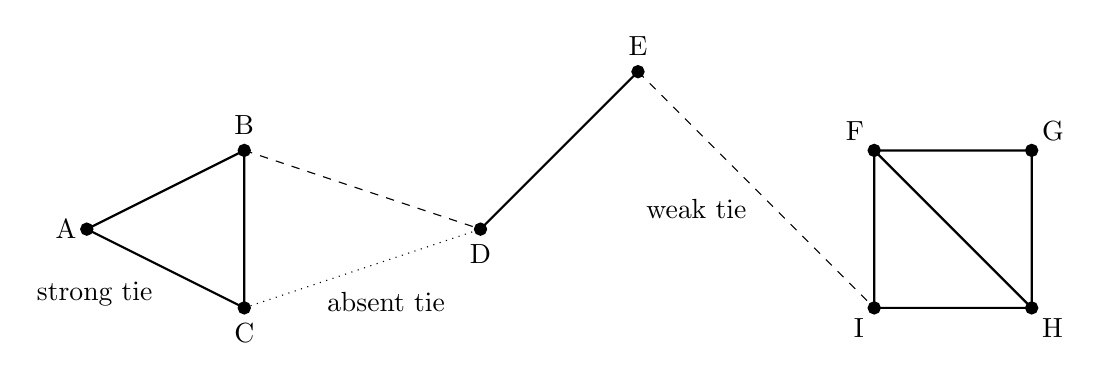
\begin{tikzpicture}
\filldraw[thick] (2,0) circle (2pt) node[below=2pt] {C} -- (0,1) circle (2pt) node[midway,below left=1pt] {strong tie} node[left] {A} -- (2,2) circle (2pt) node[above=2pt] {B} -- (2,0);
\filldraw[thick] (5,1) circle (2pt) node[below=2pt] {D} -- (7,3) circle (2pt) node[above=2pt] {E};
\filldraw[thick] (10,2) circle (2pt) node[above left] {F} -- (12,2) circle (2pt) node[above right] {G} -- (12,0) circle (2pt) node[below right] {H} -- (10,0) circle (2pt) node[below left] {I} -- (10,2);
\draw[thick] (10,2) -- (12,0);
\draw[dashed] (2,2) -- (5,1);
\draw[dashed] (7,3) -- node[midway,below left] {weak tie} (10,0);
\draw[dotted] (2,0) -- node[pos=0.6,below=8pt] {absent tie} (5,1);
\end{tikzpicture}\caption{Some examples of ties in a network.\label{fig:Example-of-ties}}
\end{figure}
With his \textquotedblleft Getting a Job\textquotedblright , Granovetter
applied those concepts to explore how people find a new job, or more
specifically, how they collect information about job opportunities.
Results from his work were consistent with the weak tie hypothesis.
It showed that the least important people in providing new job opportunities
information were friends and family. Since they interact with the
same overlapping circles of contacts, they tend to possess the same
information. This is not to say that strong ties are not important.
In fact, when a new piece of information reaches anyone in the circle,
it spreads easily and is very likely to pass on everyone with a strong
tie. However, these people are unlikely to be the source of new information
coming from distant nodes in the network. On the contrary, weak ties
with acquaintances far in the network \textendash{} e.g., in different
work situations \textendash{} make these people far more likely to
pass on new information \citep{Granovetter1974Getting-a-Job}.

\citet{Ortega2017The-Strength-of} have built upon these notions and
applied them to investigate social integration outcomes resulting
from online dating. Their work focuses on explaining the effects
of online dating on racial diversity, by virtue of the \textquotedblleft strength
of absent ties\textquotedblright . They investigate how interracial
marriages, a widely-accepted measure of social distance \citep{Qian2002Race-and-social,Wong2003Why-Do-Only-5.5},
have changed as a result of online dating penetration in the American
society. Their resulting model not only predicts almost complete racial
integration with the rise of online dating, but also slightly stronger
marriages in society overall\footnote{That is to say that, \textquotedblleft on average, marriages created
when online dating becomes available last longer than those created
in societies without this technology\textquotedblright{} \citep{Ortega2017The-Strength-of}.}. This theoretical framework is backed up by empirical U.S. data:
there is evidence that the percentage of interracial marriages has
significantly increased with the diffusion of online dating platforms
(see \prettyref{fig:Percentage-of-interr}), and that divorce rate
of marriages started online has also diminished. 
\begin{figure}[h]
\includegraphics[width=1\columnwidth]{assets/US-interracial-marriages}

\caption{Percentage of new interracial marriages in the U.S.\label{fig:Percentage-of-interr}\protect \\
{\footnotesize{}\textquotedblleft The red, green, and purple lines
represent the creation of Match.com, OKCupid, and Tinder, three of
the largest dating websites. The blue line represents a linear prediction
for 1996 \textendash{} 2015 using the data from 1967 to 1995.\textquotedblright }\protect \\
{\footnotesize{}Data retrieved from Pew Research Center analysis of
2008-2015 American Community Survey and 1980, 1990 and 2000 decennial
censuses (IPUMS).}\protect \\
{\footnotesize{}Source: \citet{Ortega2017The-Strength-of}.}}
\end{figure}
Although the authors do not claim that these phenomena are directly
caused by the spreading of online dating, they also highlight that
this observed increase in interracial marriages cannot be solely explained
by the recent changes in the American population composition. Notwithstanding
that a simple theoretical model could fail at grasping all facets
of complex social processes and at providing explanation of causality
effects, given the above, it can be concluded that the diversity of
society should anyway increase dramatically with the diffusion of
online dating.

Having scrutinised the efficiency gains at societal levels, in the
next sections we investigate the efficiency of online dating at micro-level,
by inspecting the its basic characteristics and comparing it to a
metaphorical marketplace.

\section{Principles of Online Dating}

What we elaborate in this section is supposed to refer to general
dating platforms that potentially represent all social strata existing
in society. This helpful simplification allows us to ignore specialised
dating platforms that involve only few segments of the population.

Two opposing underlying logics can be identified in the mate search
process: subconscious decisions and instrumental rationality. \citet{Willis2006First-Impressio}
found that when drawing \textquotedblleft trait inferences from the
facial appearance of other people\textquotedblright , people form
a judgement and a first impression in only 100 milliseconds. Thus
we would be induced to reject the assumptions of instrumental rationality
in the process of mate selection. However this should not be necessarily
the case, since online dating seems to be heavily influenced by such
logics of choice, exchange and competition in a market, firmly relying
on the rationale of supply and demand (see \prettyref{sec:Online-Dating-as}).

Physicality is a crucial factor in explicit partner markets like dating
platforms or nightclubs. In the context of online dating, it is primarily
expressed through the use of profile pictures, to which is given great
relevance by the user experience design. Due to the fierce competition
for attention, users must apply selective criteria of choice and reduce
complexity in decision making, both verbally and visually, hence the
paramount power that profile pictures exercise on mate choice processes.
For instance, when users are looking for a partner, they might be
tempted to flip through profiles on a dating platform, de-facto giving
substantial priority to physicality through profile pictures\footnote{Please notice that attractiveness is an important factor also for
mate choice processes that happen offline. However, other intangible
traits (and hopefully qualities) are far less likely to be perceived
online by a potential partner because of the platform design.}. Physicality is often related to the concept of erotic capital, that
\citet{Hakim2011Erotic-Capital} defines as a fourth personal asset
(added to economic, cultural, and social capital) that one should
exploit not only in mating markets, but also to powerfully advance
within society. Women allegedly have more erotic capital than men
because \textquotedblleft they work harder at it\textquotedblright{}
\citep{Hakim2010Erotic-Capital}, but this is not the only observable
gender difference in partner markets, especially in mate preference
matters.

It has been shown that both men and women strongly prefer similarity
along most attributes \textendash{} in particular for the educational
level \citep{Blossfeld2009Educational-Ass} \textendash{} but women
tend to prefer income over physical attributes more than men \citep{Hitsch2010What-Makes-You-}.
In fact, \citet{Regan2000Partner-Prefere} demonstrated that men emphasise
\textquotedblleft attributes related to sexual desirability\textquotedblright{}
more than women, who by contrast value \textquotedblleft characteristics
pertaining to social status\textquotedblright{} more than men. These
tendencies hold true also when it comes to online dating \citep{Abramova2016Gender-Differen}.
Educational homophily seems a determining factor in the online mate
choice process; it is however second to other attributes, like racial
homophily for instance. \citet{Lin2013Mate-Selection-} showed that
\textquotedblleft education does not mediate the observed racial preferences\textquotedblright{}
in the U.S. partner market. To put it in another way, white people
with a college degree are more likely to reach or respond to other
white contacts with lower educational degree than to black people
with a college degree. Moreover, it has been shown that homophily
is a strong determinant for attributes of life course (i.e., the marital
history, children etc.) and self-reported physicality (attractiveness)
and smoking habits \citep{Fiore2005Homophily-in-On,Fiore2004Romantic-Regres}.
Lastly, the concept of perfect age homophily has been partially dismissed
\textendash{} within the socially acceptable ranges of age difference
according to societal norms. \citet{Skopek2011The-gendered-dy} found
in their study that age preference shifts with age, but quite differently
between men and women. For heterosexual men, heterophily increased
with age (i.e., men prefer younger women as they age); by contrast,
for heterosexual women, age homophily increased with age (i.e., they
look for men within their same age group). All things considered,
we assume that homophily certainly plays a role in shaping mate preferences,
but it is definitely not the only significant pattern, thus we reject
the idea of one and only general logic behind online dating interactions.

Generally, men contact women more than vice versa on dating platforms;
however, a minority of women also reportedly contacted far more than
average men \citep{Scharlott1995Overcoming-Rela}. An exploratory
analysis unveiled six main motivations to use Tinder: love, casual
sex, ease of communication, self-worth validation, thrill of excitement
and trendiness \citep{Sumter2016Love-me-Tinder:}. Even though the
love motivation broadly outclassed the casual sex one, in line with
previous studies \citep[e.g.,][]{Regan2000Partner-Prefere}, \citeauthor{Sumter2016Love-me-Tinder:}
found that men are more likely to admit a casual sex motivation than
women, whereas the latter are more prone to romance and long-term
relationships. As emerged from the work of \citet{Timmermans2017To-Tinder-or-no}
on the motives to use Tinder based on the Five-Factor Model, singles
who use the app are more extraverted, open to new experiences and
less conscientious than those who do not. However, shy users are more
likely than extroverts to admit that they are using the platform to
look for love or sex, suggesting that shy users are helped by Computer-Mediated
Communication and matchmaking platforms to overcome their inhibitions
and relationship-initiation barriers \citep{Scharlott1995Overcoming-Rela}.

Due to the excess of potentially available partners, the logics of
competition (for attention) can be applied to online dating. In fact,
the actual probability of a first date are quite low. Not to mention
that the chances of early termination of communication are extremely
high, especially since not replying to a message is more broadly and
socially accepted when compared to offline social venues, like school
or family. This easy way out of a conversation becomes necessary in
a highly competitive context where actions are lead by the principle
of maximisation. However, as researches reveal, people \textquotedblleft search
surprisingly little for available marriage partners\textquotedblright{}
and they often evaluate attributes in a strongly biased way \citep{Frey1996Marriage-Parado}.
The question of whether the same applies to online partner markets
or online dating platforms help to mitigate such issues is yet to
be answered.

\subsection{Online Dating Functioning and its Effects on Behaviour}

\citet{Fiore2004Romantic-Regres} proved that the number of contact
requests sent by online daters significantly depends on the number
of contacts received. Moreover, the latter number increases the user's
mate value (see \prettyref{subsec:The-Partner-Market}). Thus it is
clear why laymen crave to be contacted by as many potential daters
as possible. As a consequence, self-presentation seems crucial to
attract other users on dating platforms but often degenerates, inducing
pressure to present themselves the most attractive as possible. To
a certain extent, this concept could be even traced back to old \textquotedblleft personal
ads\textquotedblright{} in newspapers, studied in \textquotedblleft People
as Products\textquotedblright{} by \citep{Hirschman1987People-as-Produ}.
However, this is not to say that a good first impression is unnecessary
in traditional dating environments, but it is especially important
in online dating due to technical design and low attention span.

Combined with the above reasons, the high level of uncertainty about
the authenticity of the other party enables a wide range of deceptive
practices \citep{Wang2007Cyberdating:-Mi}. These are very frequent
on online dating platforms and usually range from small discrepancies
to completely false profiles, even though the extent of such practices
is insignificant in the majority of cases \citep{Hancock2007The-Truth-about}.
False self-presentation is in fact a common rational strategy put
in place to avoid competitive disadvantage, as everyone wishes to
develop the most attractive profile. Thus it is not a result of psychological
traits, but rather a deliberate practice to defeat competition. Those
less endowed with relevant resources (i.e., with a low mate value,
see \prettyref{subsec:The-Partner-Market}) are more likely to adopt
deceptive practices in their profiles. Nonetheless, women generally
deceive less than men, and the latter are more likely to take \textquotedblleft specific
compensation of disadvantageous chances\textquotedblright{} when referring
to body characteristics (e.g small men misrepresenting their height),
according to \citet{Zillmann2011Liars-have-shor}.

One final remark, which is omnipresent both in laymen and scholars
debates, relates to infidelity. Extradyadic behaviour is common practice,
both online and offline, especially among young adults. Individuals
can engage in emotional infidelity or sexual infidelity \textendash{}
or both \citep{Blow2005Infidelity-in-c}. Some researchers explored
online infidelity through Tinder and found that the app effectively
facilitated the engagement with extraneous relationship partners \citep{Weiser2017Swiping-right:-}.
However, the debate is still open: despite these findings, \citet{Rosenfeld2017Marriage-Choice}
not only rejected the idea of online dating as a source of relationship
instability \textendash{} couples met online and offline have similar
rates of breakup \textendash{} but also found that heterosexual couples
met online have a quicker transition to marriage than those who met
offline. 

\subsection{Differences with Respect to Traditional Venues}

When compared to traditional partner markets, online dating seems
defined by smaller search friction, an expanded set of potential mates,
a higher degree of anonymity and less subject to particular social
norms\footnote{For instance, dating multiple partners offline (i.e., having interactions
with more than potential partner at a time) is often a socially disapproved
behaviour. }. Thus all matches and potential encounters are mainly guided by personal
preferences and rational intentions. Moreover, this is magnified by
the explicit function of online dating, that is to form new couples.
While in many traditional contexts, like school or neighbourhood,
couple formation is an \textquotedblleft unintended side-effect of
context-specific practice\textquotedblright{} that does not foster
\textquotedblleft a seller-buyer logic of interactions\textquotedblright ,
the main motive behind dating platforms is to look for a partner \citep{Schmitz2016The-Structure-o}.
Due to its explicit nature, dating platforms differ further from conventional
venues usually frequented by homogeneous groups of people, as they
allow users to interact with people from socially heterogeneous groups
as well. Furthermore, in case two people who interacted offline and
failed at forming a couple or relationship might continue to interact
in offline contexts, in online dating the chances of future meetings
are modest. \citet{Finkel2012Online-Dating:-} concluded that indeed
online dating significantly altered access, communication and matching
compared to offline dating, but it does not necessarily generate superior
romantic outcomes, despite some of its valuable advantages over offline
partner markets. 

\subsection{Matchmaking and Scroll-based Models\label{subsec:Matchmaking-and-Scroll-based}}

The online dating landscape is very diverse and many different functioning
models of dating platforms can be identified. A first classification
relates to the degree of specialisation: mainstream services coexist
along with more specialised services that only target a niche audience
(e.g., ethnics, single parents, seniors or younger demographics etc.)
or particular interests (e.g., adult dating, fetish, hook-ups etc.).
However, a more interesting distinction can be further outlined between
matchmaking systems and scroll-based platforms (\textquotedblleft online
dating\textquotedblright{} in general among scholars). According to
\citet{Schmitz2014The-Online-Dati}, in the first model a new user
is required to answer a comprehensive list of questions regarding
his or her personality traits and lifestyle \textendash{} along with
other questions on smoke habits, children and marriages. An algorithm
then computes a one-dimensional factor based on these pieces of information
and the system uses it to suggest potential partners to the new user.
The rationale behind this matching factor is, in most of the cases,
the similarity between the user profile with those of potential others.
A second model refers to those platforms in which potential couples
are not matched by an algorithm, but rather require the active\footnote{In reality, a passive participation is also possible if the user only
awaits for incoming contacts. } involvement of both parties in searching\footnote{I.e., browsing, hence the \textquotedblleft scroll\textquotedblright{}
action required on mobile apps.} and contacting the profiles that they personally consider interesting.
In the latter model usually new users provide only brief personal
(socio-demographic) information and the desired characteristics of
a potential partner.

\section{Online Dating as a Marketplace\label{sec:Online-Dating-as}}

From an economic standpoint, a market is a medium by which the exchange
of a certain good is facilitated with the interaction of buyers and
sellers who establish a price. A Weberian definition of market assumes
its existence whenever there is competition for the opportunities
of exchange. \citet{Becker1974A-Theory-of-Mar} supports this thesis
and applies it to couple formation processes: \textquotedblleft since
many men and women compete as they seek mates, a market in marriages
can be presumed to exist\textquotedblright . By virtue of extensive
information about a wide pool of potential mates, it seems that online
dating can be seen as strongly affected by competition that manifest
itself mainly through competition for attention and potential partners.
The marketplace metaphor, interpreted as \textquotedblleft a place
where people go to shop for potential romantic partners and to sell
themselves in hopes of creating a successful romantic relationship\textquotedblright ,
is particularly emphasised by the functioning and design of dating
platforms that often resemble e-commerce websites \citep{Heino2010Relationshoppin}.
Economic-based metaphors by which looking for a mate is seen in terms
of \textquotedblleft shopping\textquotedblright{} and consumption,
whereas potential mates as products, are common and useful to explicate
the exchange processes that happen in partner markets \citep{Bernard1990Market-Metaphor}.

This resonates with the principle of maximisation that guide actions
on online dating platforms. In fact, if users have clear intentions
when looking for a partner, they might be particularly inclined to
apply cost-benefit calculations: in other words, the search process
is grounded upon trait-oriented choices that ultimately force the
comparison of a large pool of alternative profiles \citep{Illouz2009An-Odd-and-Inse}.
As a consequence, we might argue that online dating is characterised
by relatively low transaction and search costs. The ultimate decision
of picking a partner is thus conceived through a \mbox{(quasi-)formal model}
of expected utility maximisation, by fulfilling personal mate preferences
while minimising the costs \textendash{} e.g., opportunity costs,
search costs or costs of a particular date or relationship. The choice
of offline continuation over the termination of contacts is thus realised
if the costs do not exceed the benefits. Because of the homogeneous
good exchanged\footnote{To a certain extent, online dating forces a standardising influence
on the users, since they are expected to appear as attractive and
interesting as possible. }, the inherent logics of supply and demand, exchange, competition
and conscious rational mate preferences, online dating can be seen
as a highly efficient partner market, and unusually close to the ideal
one \citep{Schmitz2016The-Structure-o}.


\subsection{The Partner Market and Mate Choice\label{subsec:The-Partner-Market}}

A partner market is usually referred to the user's field of social
interactions directed to eligible partners and pursued for mating
goals. However, in practice, identifying such a market is no easy
task, because of the intrinsic difficulty in determining what is the
object of trading in such a market. In fact, there is no uniform and
universal exchange entity in partner markets \textendash{} as opposed
to money in financial markets. Rationalist approaches require a general
utility unit that should be maximised in mate choice processes, but
assuming a common metric for all users is a pitfall. Different users
may be interested in different attributes (i.e., goods) in potential
partners\footnote{For instance, it would be erroneous to assume that a certain physical
attribute (e.g., being tall) is equally desirable by all users.}. To put it another way, it is not clear whether the (symbolic) goods
being marketed are the traits of potential mates, the potential partners
themselves, relationships or the exchange chances on dating platforms
\citep{Schmitz2016The-Structure-o}. Moreover, there could be more
than one kind of goods being bartered on the same market\footnote{Could we consider looking for a marriage, sexual satisfaction and
the fame deriving from coupling with a celebrity all the same kind
of goods? }.

One solution could be of thinking about the \textquotedblleft price\textquotedblright{}
of an actor as \textquotedblleft a function of actively and passively
approved and rejected offers\textquotedblright{} \citep{Schmitz2016The-Structure-o}.
Thus it would be possible to attach a mate value to each user of a
dating platform, defined according to his or her chances of attention
in the partner market. In some attempts at computing this metric the
number of potential partners has been used, but researchers failed
at recognising that it is too ambiguous \citep[e.g.,][]{Pawowski1999Impact-of-marke}.
\citet{Schmitz2016The-Structure-o} acknowledged that contacts received
by users with a low market value are worth less than those received
by users with a higher market value. Therefore he elaborated a new
function of mate value which takes into account the fact that different
contacts have different market values (see Equation \ref{eq:matevalue}
and Figure \ref{fig:Ego's-(black)-incoming}). 

\begin{figure}[h]
\begin{centering}
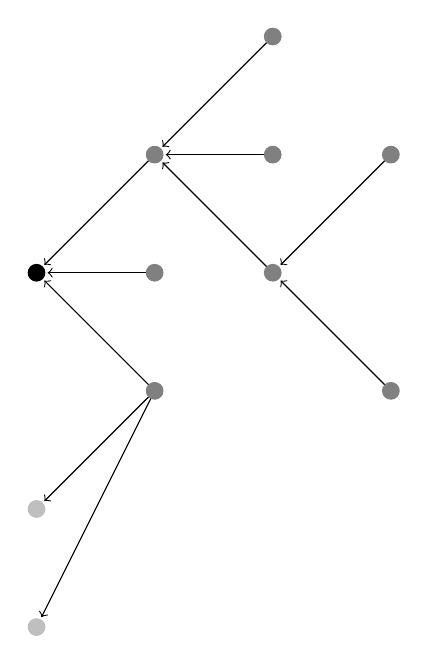
\begin{tikzpicture}[scale=1.5]
\draw[-to, shorten >=4pt] (1,2) -- (0,3);
\draw[-to, shorten >=4pt] (1,2) -- (0,1);
\draw[-to, shorten >=4pt] (1,2) -- (0,0);
\draw[-to, shorten >=4pt] (1,3) -- (0,3);
\draw[-to, shorten >=4pt] (1,4) -- (0,3);
\draw[-to, shorten >=4pt] (2,5) -- (1,4); 
\draw[-to, shorten >=4pt] (2,4) -- (1,4);
\draw[-to, shorten >=4pt] (2,3) -- (1,4);
\draw[-to, shorten >=4pt] (3,4) -- (2,3);
\draw[-to, shorten >=4pt] (3,2) -- (2,3);
\filldraw[gray!50] (0,0) circle (2pt) (0,1) circle (2pt);
\filldraw (0,3) circle (2pt);
\filldraw[gray] (1,3) circle (2pt) (1,2) circle (2pt) (1,4) circle (2pt) (2,5) circle (2pt) (2,4) circle (2pt) (2,3) circle (2pt) (3,4) circle (2pt) (3,2) circle (2pt);
\end{tikzpicture}
\par\end{centering}
\centering{}\caption{\textit{Ego}'s (black) incoming contact network.\label{fig:Ego's-(black)-incoming}}
\end{figure}
 Thus the mate prestige indicator ($MP$) is a function of the ranks
of other users contacting \textit{ego}. In fact, the number of ingoing
contacts increases \textit{ego}'s $MP$, but higher \textit{alter}
$MP$ values increase the former even more. That is to say that \textquotedblleft it
is good for one\textquoteright s mating chances to get a lot of offers;
it is even better if the offers are from potential mates who also
have good mating chances\textquotedblright .

\begin{equation}
MP_{IN}(A)=\left(1-d\right)+d\cdot\sum_{i=1}^{n}\frac{MP_{IN}(T_{i})}{C_{IN}(T_{i})}\label{eq:matevalue}
\end{equation}

\begin{spacing}{1}
\begin{verse}
{\footnotesize{}with:}{\footnotesize \par}

{\footnotesize{}$MP_{IN}(A)$ the mate prestige value of individual
$A$}{\footnotesize \par}

{\footnotesize{}$MP_{IN}(T_{i})$ the mate prestige of individuals
$T_{i}$, who contacted $A$}{\footnotesize \par}

{\footnotesize{}$C_{IN}(T_{i})$ the total number of contacts that
were established by $T_{i}$}{\footnotesize \par}

{\footnotesize{}$d$ a damping factor between 0 and 1}{\footnotesize \par}
\end{verse}
\end{spacing}

Nonetheless, readers should bear in mind that this model is nothing
more than a helpful oversimplification of complex social processes.
In reality, mental processes are far from being fully rational and
rarely follow the logics of maximisation, but rather the principle
of \textquotedblleft satisficing\textquotedblright , by which a potential
partner is picked if sufficiently meets the user's preferences \citep{Simon1956Rational-choice}.


\subsection{Choice Overload Issues}

As previously noted, when compared to traditional dating, online dating
makes available a larger pool of potential partners at once, in an
environment explicitly designed to commence communication with many
of them. Few studies have been conducted to examine whether this aspect
improved chances of romantic outcomes or lead to choice overload,
laziness in comparison strategies and ultimately to poor decisions.
In fact, it has been shown that a large choice set can overwhelm users,
leading to less efficient decisions or even in a state of choice overload
with so many alternatives that people avoid taking a decision in the
first place, rather than going through the mentally laborious process
of comparing and selecting among all the available options \citep{Finkel2012Online-Dating:-}.
This paradox of choice is a trade-off between the frustrating \textquotedblleft maximisers\textquoteright{}
desires to find the best solution\textquotedblright \footnote{As \citet{Rosenfeld2017Marriage-Choice} puts it: \textquotedblleft without
the possibility of knowing they have found the optimal solution, maximisers
become unhappy and (out of frustration) make hasty choices that make
them even more unhappy.\textquotedblright{}} and the \textquotedblleft advantage of choice\textquotedblright{}
often advertised as the greatest feature of online dating platforms
that can offer thousands of potential partners \citep{Rosenfeld2017Marriage-Choice}.

\subsection{Network Externality in a Two-sided Market}

One final remark on the functioning of online dating platforms as
marketplaces concerns indirect network effects. Network goods are
those whose utility deriving from their consumption is affected by
the number of other people consuming them (direct network effect)
or by the availability of complementary goods or networks, that depends
on the number of potential buyers (indirect network effect). In other
words, the utility increases when more people are using these products.
Thus we infer that the utility $U$ is a function of the number of
users $n$ and can be approximately computed as $U\left(n_{i}\right)=s_{i}+\alpha\cdot n_{i}$,
with $s_{i}$ the stand-alone value of the good, $\alpha$ the strength
of the network effect and $n_{i}$ the number of users $n$ in the
network $i$.
\begin{figure}[h]
\begin{centering}
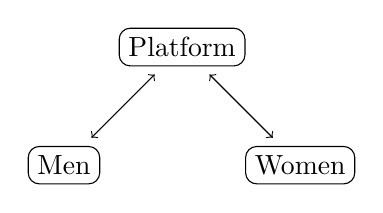
\begin{tikzpicture}[scale=1.5]
\draw[to -to, shorten >=14pt, shorten <=14pt] (0,0) -- (1,1);
\draw[to -to, shorten >=14pt, shorten <=14pt] (2,0) -- (1,1);
\filldraw (1,1) node[draw,rounded corners] {Platform} (0,0) node[draw,rounded corners] {Men} (2,0) node[draw,rounded corners] {Women};
\end{tikzpicture}
\par\end{centering}
\centering{}\caption{An example of heterosexual online dating platform as a two-sided market.\label{fig:An-example-2sided-mkt}}
\end{figure}

Many definitions of a two-sided market can be encountered in academic
research. For instance, \citealp{Evans2003Some-Empirical-} defines
it as a market in which a firm (the platform) sells two different
products to two groups of consumers, recognising that the demand of
one group depends on the demand of the other one (indirect network
effect) \textendash{} and vice versa. More generally, we define a
multi-sided platform as an organisation that creates value primarily
by enabling direct interactions between two (or more) distinct types
of affiliated customers \citep{Hagiu2015Multi-Sided-Pla}. The price
structure is also peculiar, as the allocation of the total price is
different between the different sides of the market \textendash{}
often one side is subsidised to profit from the other \citep{Rochet2003Platform-Compet}.
Since online dating platforms seem to fulfil these criteria, we are
comfortable at considering them as two-sided markets (see Figure \ref{fig:An-example-2sided-mkt}).
In fact, there are two sides or groups of customers (men and women
in the following heterosexual example, or group A and group B more
generally); the value of such platforms strictly depends on the number
of people using them and on the capacity to connect the two sides;
the usage is influenced by the allocation of prices, although price
discrimination is often ethically and logically discouraged. For instance,
by raising the price only for women on an heterosexual dating platform,
less women would use it. With less women on board, the overall value
of the service is decreased for men (and thus for the company itself
as well). Since the platform values less but the price for men has
not been changed, more men would leave, de-facto igniting a negative
feedback loop since the value of the platform would decrease also
for women as a consequence of more men leaving, and so on.


